\documentclass[b5paper]{ctexart}
\newcommand{\ts}[2]{#1\otimes #2} 
\newcommand{\tss}[3]{#1\otimes_{#2} #3} 
\newcommand{\es}[5]{$#1\xrightarrow{#2}#3\xrightarrow{#4}#5\xrightarrow{}0$} 
\newcommand{\ess}[5]{$0\xrightarrow{}#1\xrightarrow{#2}#3\xrightarrow{#4}#5\xrightarrow{}0$}
\RequirePackage{amsmath,amsthm,amsfonts,amssymb,bm,mathrsfs,wasysym}
\RequirePackage{fancyhdr}
\usepackage{exscale} 
\usepackage{relsize}
\usepackage{fourier} 
\usepackage{tikz}
\usepackage{wrapfig}
\newsavebox{\mygraphic}
\sbox{\mygraphic}{\includegraphics[totalheight=1cm]{1.ps}}
\fancypagestyle{plain}{
\fancyhf{}
\fancyhead[LE]{\usebox{\mygraphic}}
\fancyhead[LO]{\usebox{\mygraphic}}
\fancyhead[RO,RE]{ \zihao{4}宋雷~1601210073}
\fancyfoot[C]{\small -~\thepage~-}}
\RequirePackage[top=2cm,bottom=2cm,left=0.7cm,right=0.7cm]{geometry}
\renewcommand{\baselinestretch}{1.5}
\begin{document}
\pagestyle{plain}
\noindent
\zihao{4}
\begin{wrapfigure}{r}{0pt}
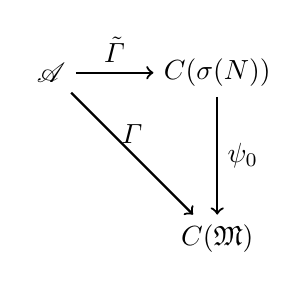
\begin{tikzpicture}[->,auto,node distance=6em, thick]
\node (X) {$\mathscr{A}$};
\node (Y) [right of=X] {$C(\sigma(N))$};
\node (T) [below of=Y] {$C(\mathfrak{M})$}; 
\draw (X) -- (Y) node[midway, above] {$\tilde{\varGamma}$};
\draw (X) -- (T) node[midway, above] {$\varGamma$};
\draw (Y) -- (T) node[midway, right] {$\psi_0$};
\end{tikzpicture}
\end{wrapfigure}
5.5.1~由$\tilde{\varGamma}$的定义,$\forall a\in\mathscr{A},(\tilde{\varGamma}a)(z)=(\varGamma a)(\psi_0^{-1}z),\forall z\in\sigma$,我们注意到$\psi_0=\varGamma N$为$\mathfrak{M}$到$\sigma(N)$上的一个同胚映射,那么右边的图表交换.而所标出的映射都是同构(胚),我们不难可以给出$\tilde{\varGamma}^{-1}$的显式表达式,$\forall \varphi\in C(\sigma(N))$,$\tilde{\varGamma}^{-1}\varphi=\varGamma^{-1}(\varphi\circ \psi_0)$那么$\forall J\in\mathfrak{M},\varphi(\varGamma N(J))=[\varGamma(\tilde{\varGamma}^{-1}\varphi)](J)$,由定理5.2.15我们有:$\sigma(N)=\{~\varGamma N(J)|J\in\mathfrak{M}~\}$,让$J$取遍$\mathfrak{M}$我们便证明了$\varphi(\sigma(N))=\sigma(\varphi(N))$.\\
(2)利用第(1)问我们有$(\psi\circ \varphi)(N)=\tilde{\varGamma}^{-1}(\psi\circ \varphi\circ\psi_0)=\psi(\varphi(N))$.\\
5.5.3~(1)由EX1可知$\sigma(P(N))=P(\sigma(N))$,所以\\
$||P(N)||=\sup~\{~|\lambda'|~|\lambda'\in \sigma{P(N)}~\}=\sup~\{~|P(\lambda)|~|\lambda \in \sigma{N}~\}$.\\
(2)我们已经验证了$\mathscr{A}_N$为交换的$C^*$代数,由EX5.4.5就可以得出结论.\\
5.5.6~注意到$N$的谱分解,我们有\\
\[N=\mathlarger{\int}_{\sigma{N}}zdE(z),N^*=\mathlarger{\int}_{\sigma{N}}\overline{z}dE(z)\]
那么$N^*N=NN^*=\mathlarger{\int}_{\sigma{N}}|z|^2dE(z)$为非负算子,那么令$P=\sqrt{N^*N}=\mathlarger{\int}_{\sigma{N}}|z|dE(z)$,令$Q=\mathlarger{\int}_{\sigma{N}}e^{-i\arg
 z}dE(z)$,那么$QQ^*=Q^*Q=I$,于是$Q$为酉算子.则$PQ=QP=\mathlarger{\int}_{\sigma{N}}zdE(z)=N$.\\
 再证唯一性,由于$P^2=N^*N$,以及正算子平方根的唯一性可知$P$是唯一的,进而$Q$也是唯一的.\\
5.5.11~必要性:其中(1)(2)由紧算子的谱集结构可知是显然的.而同时使用紧算子的谱集结构和定理4.2.10,我们可知$N$满足定理5.5.23的全部条件,即$\lambda_0\neq 0$为孤立点,$\dim \ker(\lambda_0I-N)<\infty$,所以$\lambda\in \sigma_{d}(N)$,从而存在$\lambda$的$Borel$邻域$U$,使得$\dim E(U)\mathscr{H}<\infty$.再由$\lambda\neq 0$为孤立点可知(3)成立.\\
充分性:由谱分解我们有$N=\mathlarger{\int}_{\sigma(N)}zdE(z)$,使用$Lebesgue$积分的定义,(仿造p46中$S_{\Delta}$的写法,注意由于$\varphi(z)=z$,那么值域就是定义域,所以分割定义域与分割值域是一样的.)我们可以改写积分为和式$\sum\limits_{i=1}^{\infty}\lambda_iE(\{\lambda_i\})$注意到每个$\lambda\neq 0$,有$\dim E(\{\lambda\})\mathscr{H}<\infty$,也就是说$E(\{\lambda\})$为有限秩算子.
利用上册结论:记$F(\mathscr{H})$为$Hilbert$空间上一切有限秩算子的集合,$\mathfrak{C}(\mathscr{H})$为紧算子集合,那么$\overline{F(\mathscr{H})}=\mathfrak{C}(\mathscr{H}).$所以$N=\sum\limits_{i=1}^\infty \lambda_iE(\{\lambda_i\})\in \overline{F(\mathscr{H})}=\mathfrak{C}(\mathscr{H})$,即$N$为紧算子.\\
5.5.15~先对EX14的结论做几点说明,由于我们定义的$\tau$是$B(\sigma(N))\rightarrow L(\mathscr{H})$的一个*同态,所以记号$\varphi(N)$实际上为$\varphi|_{\sigma(N)}(N)$.然后我们取$ \chi_{_\Gamma}$的一个解析开拓$\varphi$,显然有$\varphi|_{\sigma(N)}=\chi_{\sigma(N)}$.再取曲线$O,\Gamma'$使得$O$满足EX14,的条件,$\Gamma'$包含剩余的谱集.(如果解析开拓不存在,我们退而求其次,用解析函数逼近,再利用定理5.5.12,勒贝格控制收敛定理同样可以得到答案.),然后利用EX14,我们有
\[E(C)=\tau \chi_{_C}=\chi_{_{C}}(N)=\varphi_{_C}(N)=\dfrac{1}{2\pi i}\int_{\partial O}\varphi(z) (zI-N)^{-1}dz\]
注意到$\varphi(z)(zI-N)^{-1}$在由$O,\Gamma,\Gamma'$构成的区域上是弱解析的,那么
\[
\begin{array}{rll}
\dfrac{1}{2\pi i}\mathlarger{\int}_{\partial O}\varphi(z) (zI-N)^{-1}dz& =\dfrac{1}{2\pi i}\mathlarger{\int}_{\Gamma}\varphi(z) (zI-N)^{-1}dz+\dfrac{1}{2\pi i}\mathlarger{\int}_{\Gamma'}\varphi(z) (zI-N)^{-1}dz\vspace{3pt}\\
&=\dfrac{1}{2\pi i}\mathlarger{\int}_{\Gamma}(zI-N)^{-1}dz
\end{array}\]
上面右边第二个式子为零是由于$\varphi|_{\Gamma'}=0$.\\
综合两个式子我们有$E(C)=\dfrac{1}{2\pi i}\mathlarger{\int}_{\Gamma}(zI-N)^{-1}dz.$\\
6.1.1~(1)设$T\in L(\mathscr{H})$有界,若$x_n\in D(T)$满足$x_n\rightarrow 0,Tx_n\rightarrow y\in \mathscr{H}$,那么$||y||=||\lim\limits_{n\to\infty}Tx_n||=\lim\limits_{n\to\infty}||Tx_n||\leq \lim\limits_{n\to\infty}||T||||x_n||=0$,故$y=0$,由p.60注3可知$T$可闭化.\\
(2)取$T$的闭化$F$,则$R(F)\subset \overline{R(T)}$,那么$F$也是有限秩算子,再由$F|_{D(T)}=T$知$F$有界可以推出$T$有界,于是我们只需考虑$T$为有限秩闭算子的情况.当$T$为闭算子时由注3(2)可知$\ker(T)$为闭集,对于$\mathscr{H}=\ker T\oplus \ker T^{\perp}$,我们为构造投影算子$P$,使得$Px\in \ker T,(I-P)x\in\ker T^{\perp}$.不难得到$D(T)=\ker T\bigoplus (\ker T^{\perp}\cap D(T))$,$I-P$将$D(T)$映为$D(T)\cap \ker T^{\perp}$,我们需要证明$T|_{(\ker T^{\perp}\cap D(T)}$为有界算子.设$\dim R(T)=n$,那么就可以找到一组基底$\langle e_1,\cdots,e_n\rangle$线性张成$R(T)$,取定$\langle e_1,\cdots,e_n\rangle$在$\ker T^{\perp}\cap D(T)$对应的一组原像$\langle f_1,\cdots,f_n\rangle$,$Tf_i=e_i(i=1\cdots n).$我们将证明$\ker T^{\perp}\cap D(T)=\langle f_1,\cdots,f_n\rangle$,
任意的$x\in\ker T^{\perp}\cap D(T),Tx=\sum\limits_{i=1}^n\lambda_ie_i\Rightarrow T(x-\sum\limits_{i=1}^n\lambda_if_i)=0$,故$x-\sum\limits_{i=1}^n\lambda_if_i\in\ker T$,又$\ker T\cap \ker T^{\perp}=0,$于是$x-\sum\limits_{i=1}^n\lambda_if_i=0$,进而得出$ker T^{\perp}\cap D(T)=\langle f_1,\cdots,f_n\rangle$,而这是一组基也是容易证明的.这说明$T|_{(I-P)D(T)}$为有限为线性空间的线性变换,自然是有界的.那么我们便有$T=T|_{\ker T^{\perp}\cap D(T)}(I-P)$,为有界算子的复合,自然是有界的.\\
6.1.4~由于$T$是稠定对称算子,那么$T^*$总是稠定的,而$T$总是可闭化的.\\
(1)$\Rightarrow$,由$\varGamma(T^{**})=\overline{\varGamma(T)}=\varGamma(T)$,以及$T$是对称算子可知,$T=T^{**} \subset T^*$\\
$\Leftarrow$由$\overline{T}=T^{**}=T$可知$T$是闭的.\\
(2)$\Rightarrow$注意到EX6.1.3:若$T$可闭化,则$\overline{T}^*=T^*$.然后利用$T^*=\overline{T}^*=\overline{T}$,考查图我们有$\varGamma(T^{**})=\overline{\varGamma(T)}=\varGamma(\overline{T})=\varGamma(T^*),$所以$T^*=T^{**}$,而由对称性$T\subset T^*$.\\
$\Leftarrow$
$\overline{T}^*=T^*=T^{**}=\overline{T}$,这说明$\overline{T}$自伴,亦即$T$本质自伴.\\
(3)$\Rightarrow$由$T=T^*$可知,$(T^*)^*=T^*=T$,所以$T^{**}=T=T^*.$\\
$\Leftarrow$由定义可知是成立的.\\
6.1.8~(1)首先简单可测函数在$D(T)$内,不难说明它们稠于$L^2(\mathbb{R}^1)$,故$D(T)$稠于$\mathscr{H}$.\\
(2)$\forall y\in D(T^*)$,$\psi\to (y,T\psi)$为有界线性映射,由Riesz表示定理,$\exists x^*\in L^2(\mathbb{R}^1)$,使得任意的$\psi\in L^2(\mathbb{R}^1)$,有$(y,T\psi)=(x^*,\psi)$.而$(y,T\psi)=(y,(f,\psi)\psi_0)=(f,\psi)(y,\psi_0)=((y,\psi_0)f,\psi)$,那么$T^*y$的作用为为$(y,\psi_0)f$内积作用到$x$上,而定义域亦为$D(T)$.\\
6.1.12~注意这里的$a$是固定的,我们先说明$D$中元素表示为$\beta a+\sum\limits_{i=1}^n\alpha_ie_i$的方式是唯一的.若$\alpha a+\sum\limits_{i=1}^n\alpha_ie_i=\beta a+\sum \limits_{i=1}^n\beta_ie_i$(允许其中的$\alpha_i,\beta_i$取零),那么$(\alpha-\beta)a=\sum\limits_{i=1}^n(\beta_i-\alpha_i)e_i$.由$a$为无限线性组合,而等号右边为有限和,我们不难有$\alpha=\beta$,进而$\alpha_i=\beta_i$,这说明表示方法唯一,亦即$T$是良定义的.从$T(a+0)=a$可以看出$\langle a,a\rangle\in \varGamma(T)\subset\overline{\varGamma(T)}$.利用$\mathscr{H}$是可分的Hilbert空间,我们有$a=\sum\limits_{i=1}^{\infty}\alpha_ie_i$,令$a_n=\sum\limits_{i=1}^{n}\alpha_ie_i$,那么$Ta_n=T(0a+\sum\limits_{i=1}^ne_i)=0$,则$\langle a_n,0\rangle\in \varGamma(T)$.但我们有$a_n\to a$从而$\langle a_n,0\rangle\to \langle a,0\rangle$也就是说$\langle a,0\rangle\in \overline{\varGamma(T)}$.\\
6.1.15~取$u_n(x)$为
\[u_n(x)=\left\lbrace \begin{array}{ll}
\dfrac{1}{\sqrt{|x|}} & 1<|x|<n\\
0 & \text{els}e
\end{array}\right. \]
那么$\mathlarger{\int}_{-\infty}^{+\infty}u_n^2(x)dx=2\ln n<\infty$,所以$u_n(x)\in L^2(\mathbb{R}^1),$再由$\mathlarger{\int}_{-\infty}^{+\infty}x^2|u_n(x)|^2dx=2\mathlarger{\int}_{1}^{n}dx=n^2-1<\infty$可知$u_n(x)\in D(T)$,我们有$\dfrac{||Tu_n||}{||u_n||}=\dfrac{n^2-1}{2\ln n}\rightarrow \infty$,所以$T$是无界算子.\\
假设$u_n\xrightarrow{L^2}u,u_n\in D(T),u\in L^2(\mathbb{R}^1),Tu_n=xu_n\xrightarrow{L^2}y,y\in L^2(\mathbb{R}^1)$,
由实变函数可知若$u_n\xrightarrow{L^2}u$,则可取子列$u_{n_j}\to u,a.e.[\mathbb{R}^1]$.此时$xu_{n_j}\xrightarrow{L^2}y$,亦可取出子列$xu_{n_{j_k}}\to y,a.e.[\mathbb{R}^1]$,并且我们有$xu_{n_{j_k}}\to xu,a.e.[\mathbb{R}^1]$
由收敛的唯一性我们有$y=xu,a.e[\mathbb{R}^1]$,由$y\in L^2(\mathbb{R}^1)$我们有$u\in D(T)$,由p60注1我们可知$T$确实为闭算子.\\
6.1.16~存在性:我们先说明$\forall a,b\in \mathscr{H}$方程
\[\left\lbrace \begin{array}{l}
-Tx+y=a\\
x+T^*y=0
\end{array}(1)\right. ~\text{以及}~\left\lbrace \begin{array}{l}
-Tx+y=0\\
x+T^*y=b
\end{array}(2)\right.\]均存在解$x\in D(T),y\in D(T^*)$.与方程组
\[\left\lbrace \begin{array}{l}
-Tx+y=a\\
x+T^*y=b
\end{array}(3)\right.\]
对$\forall a,b\in \mathscr{H}$均存在解$x\in D(T),y\in D(T^*)$是等价的.充分性显然,必要性取方程的一组解$(x_1,y_1),(x_2,y_2)$,则$(x_1+x_2,y_1+y_2)$为第三个方程的解.必要性得证.\\
对于方程$(2)$,我们代入可得原方程等价于$(I+T^*T)x=b$有解.引理$6.3.6$说明对于稠定闭算子,$I+T^*T$是$D(T^*T)$到$\mathscr{H}$的一一在上映射,那么存在$x\in D(T^*T)\subset D(T)$,并且$y=Tx\in D(T^*)$,满足方程(2).对于方程(1),注意到$T=T^{**}$,那么$I+TT^*$为$D(T^*T)$到$\mathscr{H}$的一一在上映射,同样可以证明存在性.再由充要条件,我们可知原方程一定是有解的.\\
如果存在两组不同的解$(x_1,y_1),(x_2,y_2)$满足方程,我们令$x_0=x_1-x_2,y_0=y_1-y_2$,将两组方程相减,利用$T,T^*$均为线性算子,我们有$Tx_0=y_0,T^*y_0=-x_0$.由共轭算子的定义,我们有$\forall x\in D(T),y\in D(T^*)\Rightarrow (y,Tx)=(T^*y,x)$,那么$(y_0,y_0)=(y_0,Tx_0)=(T^*y_0,x_0)=(-x_0,x_0)$,由内积的正定性我们有$x_0=y_0=0$,即$(x_1,y_1),(x_2,y_2)$是同一组解,唯一性得证.\\
\end{document}